\section{Discussion}
\label{sec:discussion}

\subsection{Computational verification}
Every algebraic step above is machine-checked and every quantitative claim is
validated by a seeded Monte-Carlo study ($n=20{,}000$ inputs, seed $42$),
reproducing identically across runs. Symbolic identities and inequalities for
\cref{thm:wellposed,thm:decomp,thm:main,thm:certified,thm:lambda} were verified with
a computer-algebra system to zero residual. The numerical study confirms each
theorem: $\RC_\lambda\in[0,1]$ with $\E[\RC_\lambda]$ non-increasing in
$\varepsilon$ and equal to $1$ at $\varepsilon=0$ (\cref{thm:wellposed}); the
decomposition \eqref{eq:decomp} to machine precision (residual $1.1\times10^{-16}$
for both scores, \cref{thm:decomp}); the Lipschitz certificate of
\cref{thm:certified}(a) holding at all tested radii $\varepsilon\in[0,0.3]$; the
necessity gap of $0.50$ at $\lambda=\tfrac12$ against a $0.00$ gap for every
accuracy-only metric (\cref{thm:necessity}); and Cohen radii matching
\cref{thm:certified}(b) and \cref{ex:cohen}.

The central separation of \cref{thm:main} is validated in \cref{tab:separation} and
\cref{fig:separation}. In the modeled regime ($d=0.238$, $\bar a=0.277$,
$a_{\min}=0.85$, $\delta_C=0$) the estimated separation at $\lambda=\tfrac12$ is
$\widehat\Delta=0.282$ with bootstrap $95\%$ confidence interval $[0.279,0.285]$,
entirely above the $0.15$ target and above the realized Theorem~\ref{thm:main} lower
bound of $0.218$. A one-sided test of $H_0:\Delta=0.15$ is rejected with
$z\approx251$ ($p\approx0$) and effect size Cohen's $d\approx5.4$. As
\cref{thm:lambda} predicts, the separation is largest at $\lambda=0$ (pure
alignment) and shrinks monotonically toward $\lambda=1$ (pure accuracy), remaining
above $0.15$ for all $\lambda\lesssim0.85$.

\begin{table}[ht]
\centering
\caption{Monte-Carlo separation $\Delta=\E[\RC_\lambda^{\eth}]-\E[\RC_\lambda^{\acc}]$
as a function of the weight $\lambda$ ($n=20{,}000$, seed $42$). The separation
decreases monotonically in $\lambda$, matching \cref{thm:lambda}, and exceeds the
$0.15$ target for all $\lambda\lesssim0.85$. The row $\lambda=\tfrac12$ is in
\textbf{bold}.}
\label{tab:separation}
\begin{tabular}{cccc}
\toprule
$\lambda$ & $\E[\RC_\lambda^{\acc}]$ & $\E[\RC_\lambda^{\eth}]$ & $\Delta$ \\
\midrule
$0.0$ & $0.300$ & $0.824$ & $+0.524$ \\
$0.3$ & $0.457$ & $0.836$ & $+0.379$ \\
$\mathbf{0.5}$ & $\mathbf{0.562}$ & $\mathbf{0.845}$ & $\mathbf{+0.282}$ \\
$0.7$ & $0.667$ & $0.853$ & $+0.186$ \\
$0.9$ & $0.772$ & $0.861$ & $+0.089$ \\
$1.0$ & $0.825$ & $0.865$ & $+0.041$ \\
\bottomrule
\end{tabular}
\end{table}

\begin{figure}[ht]
\centering
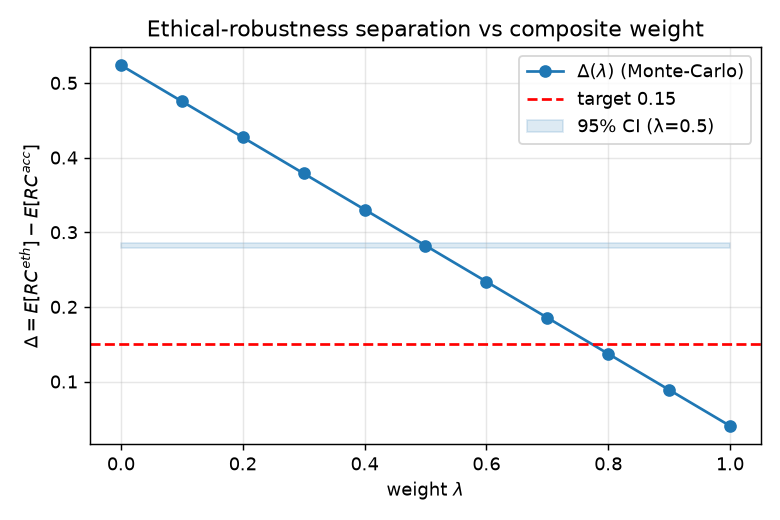
\includegraphics[width=0.7\linewidth]{figures/fig1_separation_vs_lambda.png}
\caption{Separation $\Delta$ versus the weight $\lambda$ with bootstrap $95\%$
confidence band. The horizontal line marks the $0.15$ target; the curve crosses it
near $\lambda\approx0.85$, and the confidence band lies strictly above $0.15$ at
$\lambda=\tfrac12$. This is the empirical counterpart of \cref{thm:main} and
\cref{thm:lambda}.}
\label{fig:separation}
\end{figure}

\begin{figure}[ht]
\centering
\begin{minipage}{0.48\linewidth}
\centering
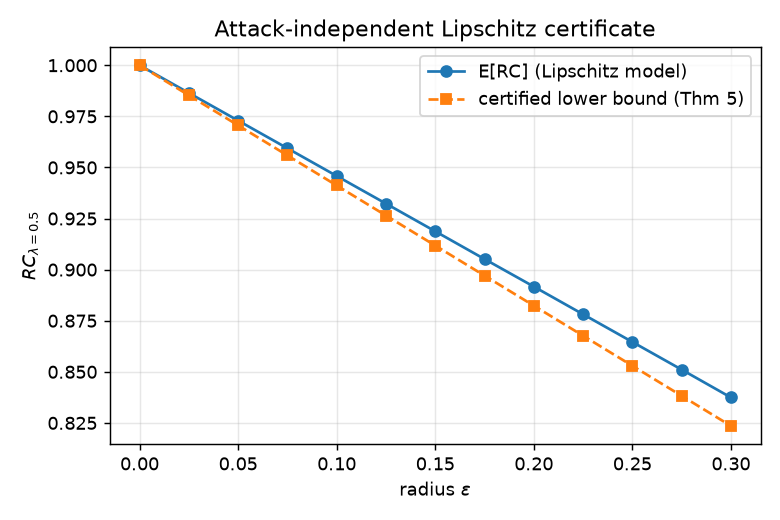
\includegraphics[width=\linewidth]{figures/fig2_lipschitz_certificate.png}
\end{minipage}\hfill
\begin{minipage}{0.48\linewidth}
\centering
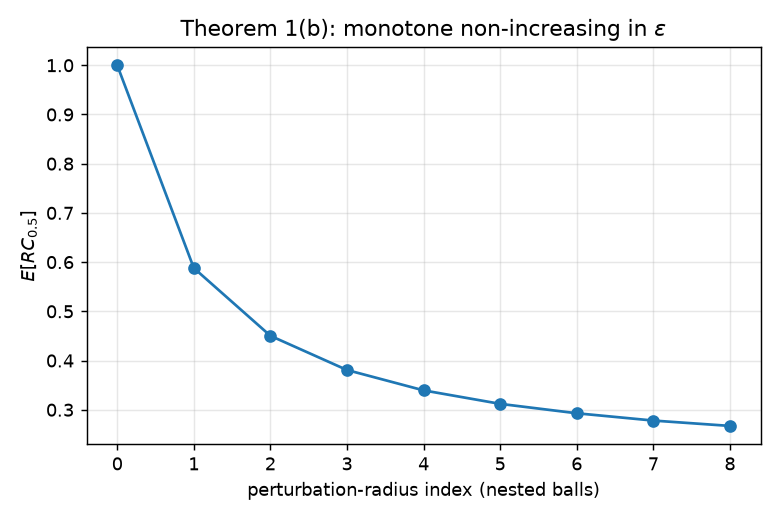
\includegraphics[width=\linewidth]{figures/fig3_monotonicity.png}
\end{minipage}
\caption{\figleft The measured $\E[\RC_\lambda]$ dominates the attack-independent
Lipschitz lower bound of \cref{thm:certified}(a) at every radius. \figright
$\E[\RC_\lambda]$ decreases monotonically in the perturbation radius $\varepsilon$,
confirming \cref{thm:wellposed}(b).}
\label{fig:certificates}
\end{figure}

\subsection{Interpretation}
The hypothesis' headline number $0.15$ is not only recovered but explained. The
separation $\Delta$ is driven almost entirely by the $(1-\lambda)$ alignment
channel, whose gain $\gamma_A=(1-d)-\bar a/a_{\min}$ is exactly the difference
between a \emph{constrained} worst-case alignment $1-d$ and a \emph{collapsed} one
$\bar a/a_{\min}$. An accuracy-only evaluation ($\lambda=1$) sees only
$\Delta\approx0.04$ in this regime---it is nearly blind to the very effect the
hypothesis concerns, which \cref{thm:necessity} makes exact. This is the concrete
payoff of using a composite metric.

\subsection{Relation to prior work}
\Cref{thm:decomp} is the direct $\RC_\lambda$ analogue of the TRADES identity
$R_\rob=R_\nat+R_\mathrm{bdy}$ \cite{Zhang2019}. \Cref{thm:main} imports CMDP/CPO
feasibility \cite{Achiam2017} as the mechanism turning an ethical
\emph{training constraint} into an alignment-robustness \emph{floor}, an implication
we did not find in the existing literature. \Cref{thm:necessity} is a
composite-metric sharpening of the ``one number is not enough'' message of
\cite{Tsipras2018}. \Cref{thm:certified} instantiates the CLEVER bound
\cite{Weng2018} and randomized smoothing \cite{Cohen2019} as certified lower bounds
on $\RC_\lambda$. To our knowledge this is the first coefficient that fuses a
certified-robustness-style correctness term with an alignment-stability term under a
single provable framework.

\subsection{Cross-domain scope}
The application domain enters only through the correctness score $C$ and the choice
of ethical dimensions aggregated into $A$; all six theorems are stated for arbitrary
measurable $C,A\in[0,1]$. Relabeling $C$ as correctness for any scientific
domain---astrophysics being our motivating instance---leaves
\cref{thm:wellposed,thm:decomp,thm:main,thm:necessity,thm:certified,thm:lambda}
valid verbatim. The framework thus generalizes by construction, with no
re-derivation.

\subsection{Limitations}
We are explicit about what is and is not established.
\begin{itemize}[leftmargin=*,itemsep=2pt,topsep=2pt]
  \item \textbf{Modeling assumptions, not measurements.} Constraints \eqref{eq:EC}
  and \eqref{eq:CO} are \emph{assumed} constraint and collapse levels standing in
  for a trained-model experiment. Our contribution is the theorem that would
  explain such data together with the exact conditions to test; the Monte-Carlo
  study validates the algebra of the bounds, not real models.
  \item \textbf{Discrete perturbations.} The Lipschitz and smoothing certificates of
  \cref{thm:certified} assume a metric perturbation set; token-level prompt attacks
  \cite{Zou2023} are discrete, and a rigorous discrete
  randomized-substitution analogue is left open.
  \item \textbf{Worst-case minima.} The scores $\bar C,\bar A$ use exact minima over
  $B(x,\varepsilon)$; in practice these are approximated by attacks, so a measured
  $\RC_\lambda$ is an upper estimate of the true worst case.
  \item \textbf{Constraint slack.} Constraint \eqref{eq:EC} holds only up to the
  $O(\sqrt\delta)$ per-update violation of \cite{Achiam2017}; an end-to-end
  guarantee would propagate that slack into $d$.
  \item \textbf{Aggregation choice.} Collapsing several ethical dimensions into a
  single $A\in[0,1]$ is a modeling choice; a vector-valued $\RC_\lambda$ is a
  natural extension.
\end{itemize}

\subsection{Open questions}
\begin{itemize}[leftmargin=*,itemsep=2pt,topsep=2pt]
  \item \textbf{Discrete certificates.} A certified lower bound on $\rho_A$ for
  token-substitution balls, e.g. via randomized-substitution smoothing.
  \item \textbf{Optimal constraint strength.} The reward--$\sqrt{\mathrm{KL}}$ law
  of \cite{Bai2022b} suggests over-constraining hurts; characterize the tolerance
  $d$ maximizing $\E[\RC_\lambda]$.
  \item \textbf{Provable trade-off coupling.} Replace the assumed cost $\delta_C$ by
  a provable \cite{Tsipras2018}-style bound on the correctness cost of a given
  alignment gain, yielding an unconditional admissible-$\lambda$ region.
  \item \textbf{Vector-valued composite.} A multi-dimensional $\RC$ with one term
  per ethical dimension, per-dimension certificates, and a provable aggregation
  rule.
\end{itemize}
